\documentclass[preprint]{revtex4-2}

\usepackage{amsmath}    % need for subequations
\usepackage{graphicx}   % need for figures
\usepackage{verbatim}   % useful for program listings
\usepackage{color}      % use if color is used in text
\usepackage{subfigure}  % use for side-by-side figures
\usepackage{hyperref}   % use for hypertext links, including those to external
\raggedbottom           % don't add extra vertical space
\begin{comment}
\pagestyle{empty}       % use if page numbers not wanted
\end{comment}

\bibliographystyle{apsrev4-2}

\begin{document}

\title{
    TensorAlloy: a highly efficient atomistic neural network program for alloys
}
\author{Xin Chen}
\author{Xing-Yu Gao}
\author{Ya-Fan Zhao}
\author{De-Ye Lin}
\email{lindeye0716@163.com}
\author{Wei-Dong Chu}
\author{Hai-Feng Song}
\email{song\_haifeng@iapcm.ac.cn}
\affiliation{
    Institute of Applied Physics and Computational Math, 
    Beijing 100088, China}
\affiliation{
    CAEP Software Center for High Performance Numerical Simulation, 
    Beijing 100088, China}


\begin{abstract}
Atomistic modeling is important for studying physical and chemical properties of
materials. Recently, machine learning interaction potentials have gained much 
more attentions as they can provide density functional theory level predictions 
within negligible time. Currently, the symmetry function descriptor based 
atomistic neural network is the most widely used model for modeling alloys. 
To precisely describe complex potential energy surfaces, integrating advanced 
metrics, such as force or virial stress, into training can be of great help. 
However, the traditional way to construct a 
machine learning model computation graph starts from pre-computed descriptors, 
but not positions, due to technial challenges. Thus, deriving analytical atomic 
force and virial stress of a machine learning model becomes quite difficult as 
the partial derivations of descriptors with respect to positions need separate 
implementations, which requires plenty of efforts and its efficiency can not be 
guaranteed.
In this paper, we designed a new method, named the virtual atom approach, for 
implementing the symmetry function descriptor and the corresponding atomistic 
neural networks. With the virtual atom approach, we are able to build 
computation graph from atomic positions \textemdash but not descriptors 
\textemdash to total energy directly, thus asking modern machine learning 
platforms to compute atomic force and virial stress becoming possible. We also 
derived a simple and machine learning friendly equation for calculating virial 
stress. All these new algorithms have been implemented in our Python package, 
TensorAlloy. TensorAlloy supports constructing machine learning interaction 
potentials for both \textit{molecules} and \textit{solids} and one hour is 
sufficient for TensorAlloy to obtain models with state-of-art level accuracy.
\end{abstract}

\maketitle

\newcommand{\tensoralloy}{\textbf{TensorAlloy}}

% % % % % % % % % % % % % % % % % % % % % % % % % % % % % % % % % % % % % % % %
% 
% Section 1. Introduction
%
% % % % % % % % % % % % % % % % % % % % % % % % % % % % % % % % % % % % % % % %
\newpage

\section{Introduction}

Atomistic simulations (\textit{ab initio} calculation, classic molecular 
dynamics simulation (MD), etc) are powerful tools for studying physical and 
chemical properties of materials. To obtain reliable simulation results, 
atomistic interactions must be properly described. The very accurate 
\textit{ab initio} and quantum chemical methods have gain significant 
improvements over the past decades but their applicabilities are restricted by 
computation expenses. Physical model based empirical potentials, such as the 
embedded-atom method\cite{eam-1,eam-2,eam-3,eam-4,eam-5} or its variants (
modified embedded-atom method\cite{eam-5,meam-1,meam-2,meam-3}, 
angular-dependent interaction potential\cite{adp-1,adp-2,adp-3}, etc), are much 
more popular for long-time simulation because of their reasonable accuraty and 
acceptable costs. 
However, designing empirical potentials and optimizing parameters for 
alloys are still challenging tasks\cite{eam-5, adp-2, SNAP_2018}. 

In the past few years, machine learning (ML) has become one of the most 
influential topic in almost all fields of science. A lot of effort has been made 
by various physicists to explore the possiblity of using ML models \textemdash 
instead of traditional empirical potentials \textemdash to describe atomistic 
interactions during MD simulations\cite{kCON,SchNet,DTNN,SNAP_2018,SNAP_Mo_2017,
ANI,TensorMol}. ML potentials are much easier to design and 
optimize. With sufficient training data, ML models can achieve similar or even 
better performances compared with density functional theory.
The symmetry function based atomistic neural network (ANN) model, first proposed 
by Parinello and Behler in 2007\cite{Behler,Behler2,Behler3,Behler4,Behler1}, 
is still the most widely used method for \textit{solids} and its effectness and 
accuracy has been proven by several 
works\cite{Behler-solids-lzp-1,Behler-alloy-1,Behler-alloy-2, Behler-alloy-3}.
Until now, various ML implementations\cite{AMP,ANI,TensorMol} have been 
published by researchers. The Amp\cite{AMP} package, developed by Peterson's 
group, is the first open-source framework that implements the symmetry function 
descriptor. Amp can be used to learn interaction potentials for both 
\textit{molecules} and \textit{solids} and it has successfully powered quite a 
few researches since 2016\cite{Amp-works-hammer,amp-work-1}. ANI\cite{ANI} and 
TensorMol\cite{TensorMol} are also symmetry function based packages but they 
mainly focus on \textit{molecules}.

In order to precisely model atomistic interactions, both total energy and atomic 
forces are necessary. For \textit{solids}, the virial stress tensor is also an
essential metric. However, integrating force and stress into the loss function 
is not an easy task. The machine learning approaches favor vectorizable 
operations but the calculations of atomic descriptors are typically complicated 
so that many traditional ML packages (Amp, kCON, etc) choose to pre-compute 
descriptors and only build computation graph from descriptors to total energy. 
This approach can significantly reduce technical difficulty and works very well 
if only total energy is considered in the loss function. But to fit atomic 
forces, numerous codes must be written manually, such as the derivation of 
descriptors with respect to positions. Although the derivation is theoretically
clear, the implementation is challenging and the efficiency can not be 
guaranteed.

Recently, machine learning platforms (TensorFlow\cite{tensorflow}, 
PyTorch\cite{pytorch}, MXNet\cite{MXNet}, etc) have gain significant 
developments. These modern machine learning frameworks can fully take advantage 
of GPUs for acceleration. The automatic differentiation capability brings a new 
route for devloping ML models capable of predicting energy, force and stress as 
we may 'let' ML platforms to handle the calculations of force and stress because 
these metrics can be derived from positions and total energy directly. To 
achieve this, a direct computation graph from positions to total energy must be
built. Thus, the problem becomes: how to design such route?

In this work, we propose a new algorithm, named the virtual atom approach, to 
implement the symmetry function descriptor and the ANN model based on 
TensorFlow. This algorithm is very suitable for parallel execution. With this 
approach, stochastic gradient descent (SGD) based mini-batch training can be 
adopted. We also derive a general and vectorizable expression for computing 
virial stress for arbitrary ANN model. All these algorithms have been 
implemented in our Python program: \tensoralloy{}. 

This paper is organized as follows. Section \ref{section:theory} introduces the 
theory of the symmetry function descriptor and the ANN framework. Section 
\ref{section:method} describes the virtual atom approach and a modified ANN 
model used by \tensoralloy{}. Section \ref{section:discussions} displays 
performances of \tensoralloy{} on two public datasets. The appendix 
\ref{section:appendix} gives derivation and implementation details of key 
algorithms. The \tensoralloy{} program can be obtained on request.

% % % % % % % % % % % % % % % % % % % % % % % % % % % % % % % % % % % % % % % %
% 
% Section 2. Theory
%
% % % % % % % % % % % % % % % % % % % % % % % % % % % % % % % % % % % % % % % %
\section{Theory}
\label{section:theory}

\newcommand{\rijn}{r_{ij\mathbf{n}}}

In the atomistic neural network (\textbf{ANN}) framework, the total energy, 
$E^{total}$, of a structure with $N$ atoms, is the sum of all atomic energies:
\begin{equation}
\label{eq:general_e_total}
E^{total} = \sum_{i}^{N}{E_i}
\end{equation}
where $E_{i}$, the energy of atom \textit{i}, is the output of the neural 
network $\mathbf{NN}_{el}$ for element $el$:
\begin{equation}
E_i = \mathbf{NN}_{el}\left( \mathbf{G}_i \right)
\end{equation} 
Here $\mathbf{G}_i$ is a vector representing atomic descriptors of atom $i$. 
$\mathbf{G}_i$ typically only depends on local environments, i.e.  
neighbors of atom $i$:
\begin{equation}
\mathbf{G}_i = F_G(\left\{ \rijn, |\rijn| < r_c\right\} )
\end{equation}
where $F_G$ can be arbitrary function, $r_c$ is the cutoff radius and $\rijn$ is 
the interatomic distance considering the periodic boundary conditions: 
\begin{equation}
    \label{eq:rijn}
    \rijn = \Vert \mathbf{r}_i^{(0)} - \mathbf{r}_j^{(0)} + 
    \mathbf{n}^T \mathbf{h} \Vert
\end{equation}
where $\mathbf{r}_i^{(0)}$ and $\mathbf{r}_j^{(0)}$ denote positions of $i$ and 
$j$ in the primitive cell, $\mathbf{n}$ is a column vector specifying the cell 
shifts along $(X,Y,Z)$ directions 
\begin{equation}
    \label{eq:ij_shift}
    \mathbf{n} = \begin{pmatrix}
        n_x \\
        n_y \\
        n_z
    \end{pmatrix}
\end{equation}
and $\mathbf{h}$ is the \textbf{row-major} $3 \times 3$ lattice tensor:
\begin{equation}
    \label{eq:lattice}
    \mathbf{h} = \begin{pmatrix}
        h_{xx} & h_{xy} & h_{xz} \\
        h_{yx} & h_{yy} & h_{yz} \\
        h_{zx} & h_{zy} & h_{zz} \\
    \end{pmatrix}
\end{equation}

\newcommand{\rijna}{r_{ij\mathbf{n_1}}}
\newcommand{\rikna}{r_{ik\mathbf{n_2}}}
\newcommand{\rjkna}{r_{jk\mathbf{n_3}}}

There are many choices of $F_G$. The symmetry function descriptor, proposed 
by Parinello and Behler in 2007\cite{Behler}, is currently the most widely used 
atomic descriptor, especially for alloys. The symmetry function descriptor 
consists of two sets of invariant (tranlational, rotational and permutational) 
functions: the radial symmetry function $\mathbf{G}^{(2)}$ and the angular 
symmetry function $\mathbf{G}^{(4)}$:
\begin{align}
\label{eq:G2}
\mathbf{G}^{(2)}_i(\eta, R_s) = & \sum_{j \neq i}{
    \sum_{\mathbf{n}}{g_2 (\eta, i, j, R_s)}
} \\
\label{eq:G4}
\mathbf{G}^{(4)}_i(\beta, \gamma, \zeta) 
= & 2^{1-\zeta}\sum_{j, k\neq j, k\neq i}{
    \sum_{\mathbf{n}_1}{\sum_{\mathbf{n}_2}{\sum_{\mathbf{n}_3}{
        g_4(\beta, \gamma, \zeta, 
          i, j, k, 
          \mathbf{n}_1, \mathbf{n}_2, \mathbf{n}_3)
    }}}
} \\
\label{eq:g2}
g_2 = & \exp\left\{-\frac{\eta(\rijn - R_s)^2}{r_c^2} \right\}
\cdot f_c(\rijn) \\
g_4 = & \left( 1 + \gamma\cos\theta \right)^\zeta 
    \exp \left\{ -\frac{\beta(\rijna^2 + \rikna^2 + \rjkna^2)}{r_c^2} \right\}
f_c(\rijna)f_c(\rikna)f_c(\rjkna)
\end{align}
where $\eta$, $R_s$, $\beta$, $\gamma$ and $\zeta$ are empirically chosen 
parameters, $f_c(r)$ is a cutoff (damping) function and its original form is:
\begin{equation}
\label{eq:fc_origin}
f_c(r) =
    \begin{cases}
    0 & \text{$r > r_c$} \\
    \frac{1}{2} + \frac{1}{2}\cos\left(r / r_c \cdot \pi \right) & 
    \text{$r \leq r_c$}
    \end{cases}
\end{equation}
and $r_c$ is the cutoff radius. $R_s$ may be fixed to zero \cite{AMP}. 
Equation \eqref{eq:fc_origin} can be further transformed to a vectorized 
expression:
\begin{equation}
\label{eq:fc}
f_c(r) = \frac{1}{2}\left( 
    1 + \cos\left[ \min(\frac{r}{r_c}, 1) \pi \right] 
\right)
\end{equation} 
and $\cos\theta$ also has a vectorized form:
\begin{equation}
\cos\theta = \frac{\rijna^2 + \rikna^2 - \rjkna^2}{2 \rijna \cdot \rikna}
\end{equation}
The summations in $\mathbf{G}^{(2)}$ and $\mathbf{G}^{(4)}$ should go over all 
neighbors within $r_c$. 

Analytical atomic forces can be obtained directly by computing the first-order 
derivative of $E^{total}$ with respect to $\mathbf{r}_{a}^{(0)}$ where $a$ is an 
index:
\begin{equation}
\label{eq:dEdr}
f_a = -\frac{\partial E^{total}}{\partial \mathbf{r}_a^{(0)}}
\end{equation}
According to the chain rule, we can expand Equation \ref{eq:dEdr}:
\begin{align}
\frac{\partial E^{total}}{\partial \mathbf{r}_a^{(0)}} = & \sum_{i}^{N}{
    \frac{
        \partial\mathbf{NN}_{el}(\mathbf{G}_i)}{
        \partial \mathbf{r}_a^{(0)}}} \nonumber \\
= & \sum_{i}^{N}{\sum_{l}^{N_G}{
    \frac{\partial \mathbf{NN}_{el}(\mathbf{G}_i)}{\partial G_{il}}
    \cdot
    \frac{\partial G_{il}}{\partial \mathbf{r}_{a}^{(0)}}
}}
\end{align}
and 
\begin{align}
\frac{\partial G_{il}^{(2)}}{\partial \mathbf{r}_{a}^{(0)}} = & \sum_{j \neq i}{
    \sum_{\mathbf{n}}{
        \frac{\partial g_2}{\partial \rijn}
        \cdot
        \frac{\partial \rijn}{\partial r_k^{0}}
    }
} \\
\frac{\partial G_{il}^{(4)}}{\partial \mathbf{r}_{a}^{(0)}} = &
2^{1 - \zeta}\sum_{j, k \neq j, k \neq i}{
    \sum_{\mathbf{n}_1}{\sum_{\mathbf{n}_2}{\sum_{\mathbf{n}_3}{
        \left(
            \frac{\partial g_4}{\partial \rijna}
            \frac{\partial \rijna}{\partial \mathbf{r}_{a}^{(0)}} + 
            \frac{\partial g_4}{\partial \rikna}
            \frac{\partial \rikna}{\partial \mathbf{r}_{a}^{(0)}} + 
            \frac{\partial g_4}{\partial \rjkna}
            \frac{\partial \rjkna}{\partial \mathbf{r}_{a}^{(0)}}
        \right)
    }}}
}
\end{align}

The derivations are theoretically straightforward but their implementations are 
challenging \cite{AMP}. Later we will provide a new approach to address this 
problem.

The $3 \times 3$ virial stress tensor $\epsilon$ is an important metric to 
describe solids under deformation or external pressure. For arbitrary many-body 
interaction potentials, $\epsilon$ can be calculated with the following equation
\cite{lammps_stress}:
\begin{equation}
\label{eq:stress_lammps}
V \cdot \epsilon = \left(-\sum_{i=1}^{N}{\mathbf{r}_i^{(0)} \otimes f_i} - 
\sum_{\mathbf{n}}{\mathbf{h}^T\mathbf{n}} \otimes 
\sum_{i=1}^{N}{F^{\prime}_{i\mathbf{n}}}
\right)^T
\end{equation}
where $V$ is the volume, $\otimes$ indicates tensor product, $f_i$ is the total 
force acting on atom $i$ and $F^{\prime}_{i\mathbf{n}}$ is the partial force. 
Until now, most machine learning force-field models focus on fitting total 
energy and atomic forces, very few of them\cite{DeePMD,DeePMD_rl,DeePMD_kit} had 
attempted to include stress in their loss functions. 
The current expression of Equation \ref{eq:stress_lammps} is not very compatible 
with NN or other ML potentials since the partial forces are difficult to compute 
with vectorized operations. To resolve this issue, we derived an equivalent form 
of Equation \ref{eq:stress_lammps}:
\begin{equation}
\label{eq:stress}
V \cdot \epsilon = -F^{T} R + 
\left(\frac{\partial E^{total}}{\partial \mathbf{h}}\right)^T \mathbf{h}
\end{equation}
where $R$ is the $N \times 3$ positions matrix and $F$ is the 
corresponding total forces matrix. The new equation can be easily implemented 
with simple matrix operations. The detailed derivation is given in the appendix.

% % % % % % % % % % % % % % % % % % % % % % % % % % % % % % % % % % % % % % % %
% 
% Section 3. Method
%
% % % % % % % % % % % % % % % % % % % % % % % % % % % % % % % % % % % % % % % %
\section{Method}
\label{section:method}

\newcommand{\nmax}{
    N_{\mathrm{Ni}}^{\mathrm{max}}+N_{\mathrm{Mo}}^{\mathrm{max}}
}
\newcommand{\nijmax}{N_{ij}^{\mathrm{max}}}
\newcommand{\nijkmax}{N_{ijk}^{\mathrm{max}}}

In this section we will describe details of \tensoralloy{}: the virtual atom 
approach, the atomic residual potential and the loss function. 
The Ni-Mo binary alloy system will be used as the example to show this 
algorithm. The virtual atom approach is built upon TensorFlow. For simplicity, 
only radial symmetry function related algorithms are visualized in the figures.

\subsection{The virtual atom approach}
\label{section:virtual_atom_approach}

Fig \ref{fig:algo1} shows the initialization procedure of the virtual atom 
approach. The cutoff radius $r_{cut}$ must be fixed. The first step is to go 
through the entire dataset and determining four prerequisite constants: 
$N_{ij}^{\mathrm{max}}$, $N_{ijk}^{\mathrm{max}}$, 
$N_{\mathrm{Ni}}^{\mathrm{max}}$ and $N_{\mathrm{Mo}}^{\mathrm{max}}$. 
Here $N_{ij}^{\mathrm{max}}$ represents the maximum number of neighbor pairs 
and $N_{ijk}^{\mathrm{max}}$ represents the maximum number of triples in 
arbitrary structure. 
$N_{ij}^{\mathrm{max}}$ and $N_{ijk}^{\mathrm{max}}$ only depend on 
$r_{cut}$. The associated codes are given in the appendix.
$N_{\mathrm{Ni}}^{\mathrm{max}}$ and $N_{\mathrm{Mo}}^{\mathrm{max}}$ indicate 
the maximum appearances of Ni and Mo in any structure, respectively. 
With $N_{\mathrm{Ni}}^{\mathrm{max}}$ and $N_{\mathrm{Mo}}^{\mathrm{max}}$, 
the global symbol list (GSL) can be created. GSL defines the global reference 
of this dataset and must be maintained during entire training. Then we can 
construct \textit{offsets}. This vector marks the starting indices of the 
\textbf{ordered} interaction pairs (e.g. Ni-Mo) and triples (e.g. Ni-Ni-Mo). 
The order of the interactions must be maintained as well.

\begin{figure}[h!]
\centering
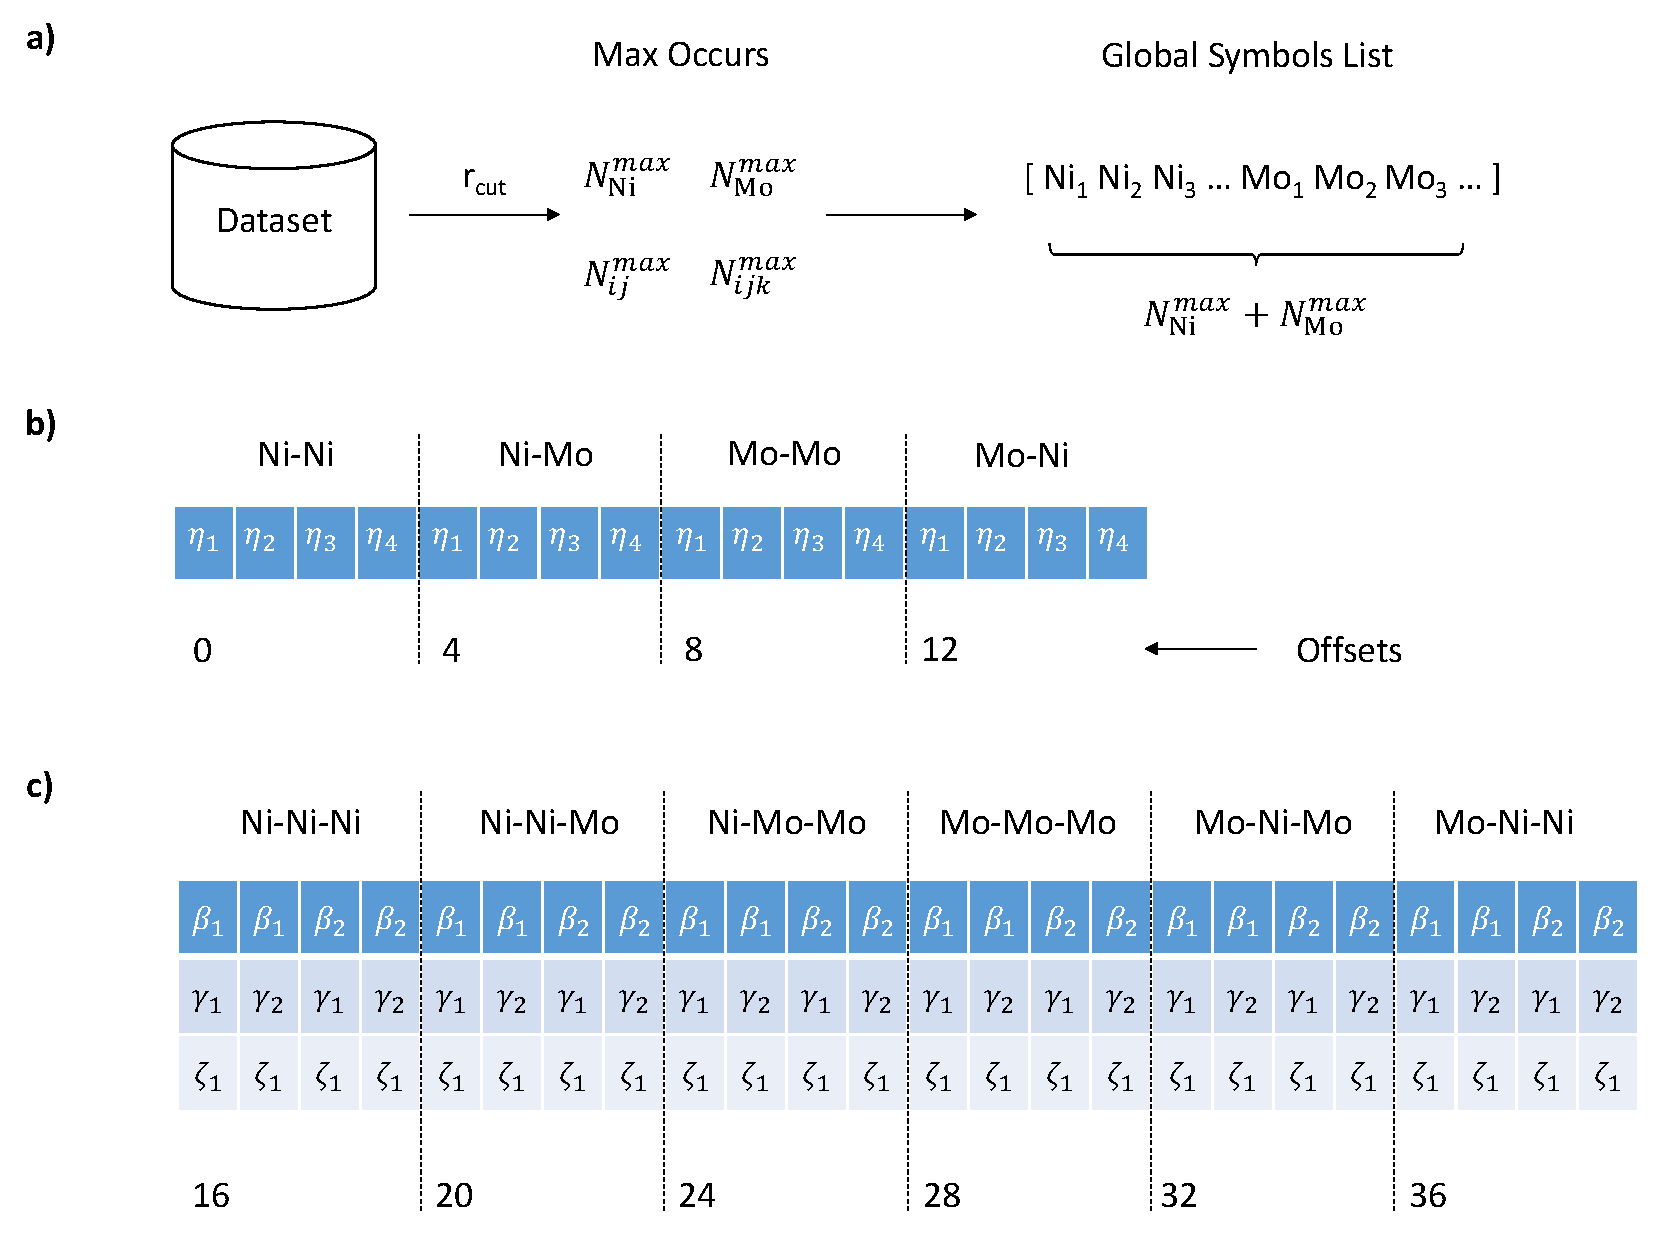
\includegraphics[scale=0.5]{figures/Fig1-prepare.pdf}
\caption{\label{fig:algo1} The initialization step. 
\textbf{a)} describes the detections of $N_{\mathrm{Ni}}^{\mathrm{max}}$, 
$N_{\mathrm{Ni}}^{\mathrm{max}}$, $N_{ij}^{max}$, $N_{ijk}^{max}$ and the global
symbols list.
The \textit{offsets} of radial and angular functions and their corresponding 
symmetry function parameters are in \textbf{b)} and \textbf{c)}, respectively.
}
\end{figure}

Fig \ref{fig:algo2} shows the algorithm to construct the radial mapping matrix
$g_{\mathrm{map}}^2$ which plays a key role in building the computation graph 
(Fig \ref{fig:algo3}). This algorithm starts from the $N \times 3$ local 
positions matrix \textbf{R}. Here 'local' means original and 'global' means GSL. 
The first step is to find all neighbor pairs: $\mathbf{n}$, $i^{(0)}$ and 
$j^{(0)}$. This can be done by the 
\href{https://wiki.fysik.dtu.dk/ase/ase/neighborlist.html}{neighbor\_list} 
routine of ASE\cite{ase}. $\mathbf{n}$ is a $N_{ij} \times 3$ matrix 
representing the periodic boundary shift vectors where $N_{ij}$ is the total 
number of interaction pairs within $r_{cut}$.
Both $i^{(0)}$ and $j^{(0)}$ are $N_{ij}\times 1$ column vectors representing 
the indices of $i$ and $j$ of Equation \ref{eq:rijn}. 
$\mathbf{t}$ is a manually-created $N_{ij}\times 1$ column vector storing the 
types \textemdash represented by integers \textemdash of the corresponding 
interaction pairs.

The second step is to convert the local indices, $i^{(0)}$ and $j^{(0)}$, to 
global indices based on GSL and then \textbf{increase their values by one}. 
By padding with zeros, we can finally get the $N_{ij}^{\mathrm{max}} \times 3$ 
matrix $\mathbf{n_g}$ and $N_{ij}^{\mathrm{max}} \times 1$ column vectors 
$i^{(0)}_{\mathrm{+,g}}$, $j^{(0)}_{\mathrm{+,g}}$ and 
$\mathbf{t}_{\mathrm{g}}$. The increment is extremely important because the 
indices of all padded 'virtual' or 'dummy' atoms are fixed to 0.

The last step is to construct $g_{\mathrm{map}}^{(2)}$, which should be a 
$N_{ij}^{\mathrm{max}} \times 2$ matrix. Its first column is just 
$i^{(0)}_{\mathrm{+,g}}$ and its second column are corresponding offset values 
of $\mathbf{t}_{\mathrm{g}}$. $g_{\mathrm{map}}^{(2)}$, 
$j^{(0)}_{\mathrm{+,g}}$ and $\mathbf{n_g}$ can be pre-computed and cached. 
The algorithm to build $g_{\mathrm{map}}^{(4)}$ for angular symmetry functions 
is similar but too complicated to visualize. Thus, we provide a Python 
implementation in the appendix. 

\begin{figure}[h!]
\centering
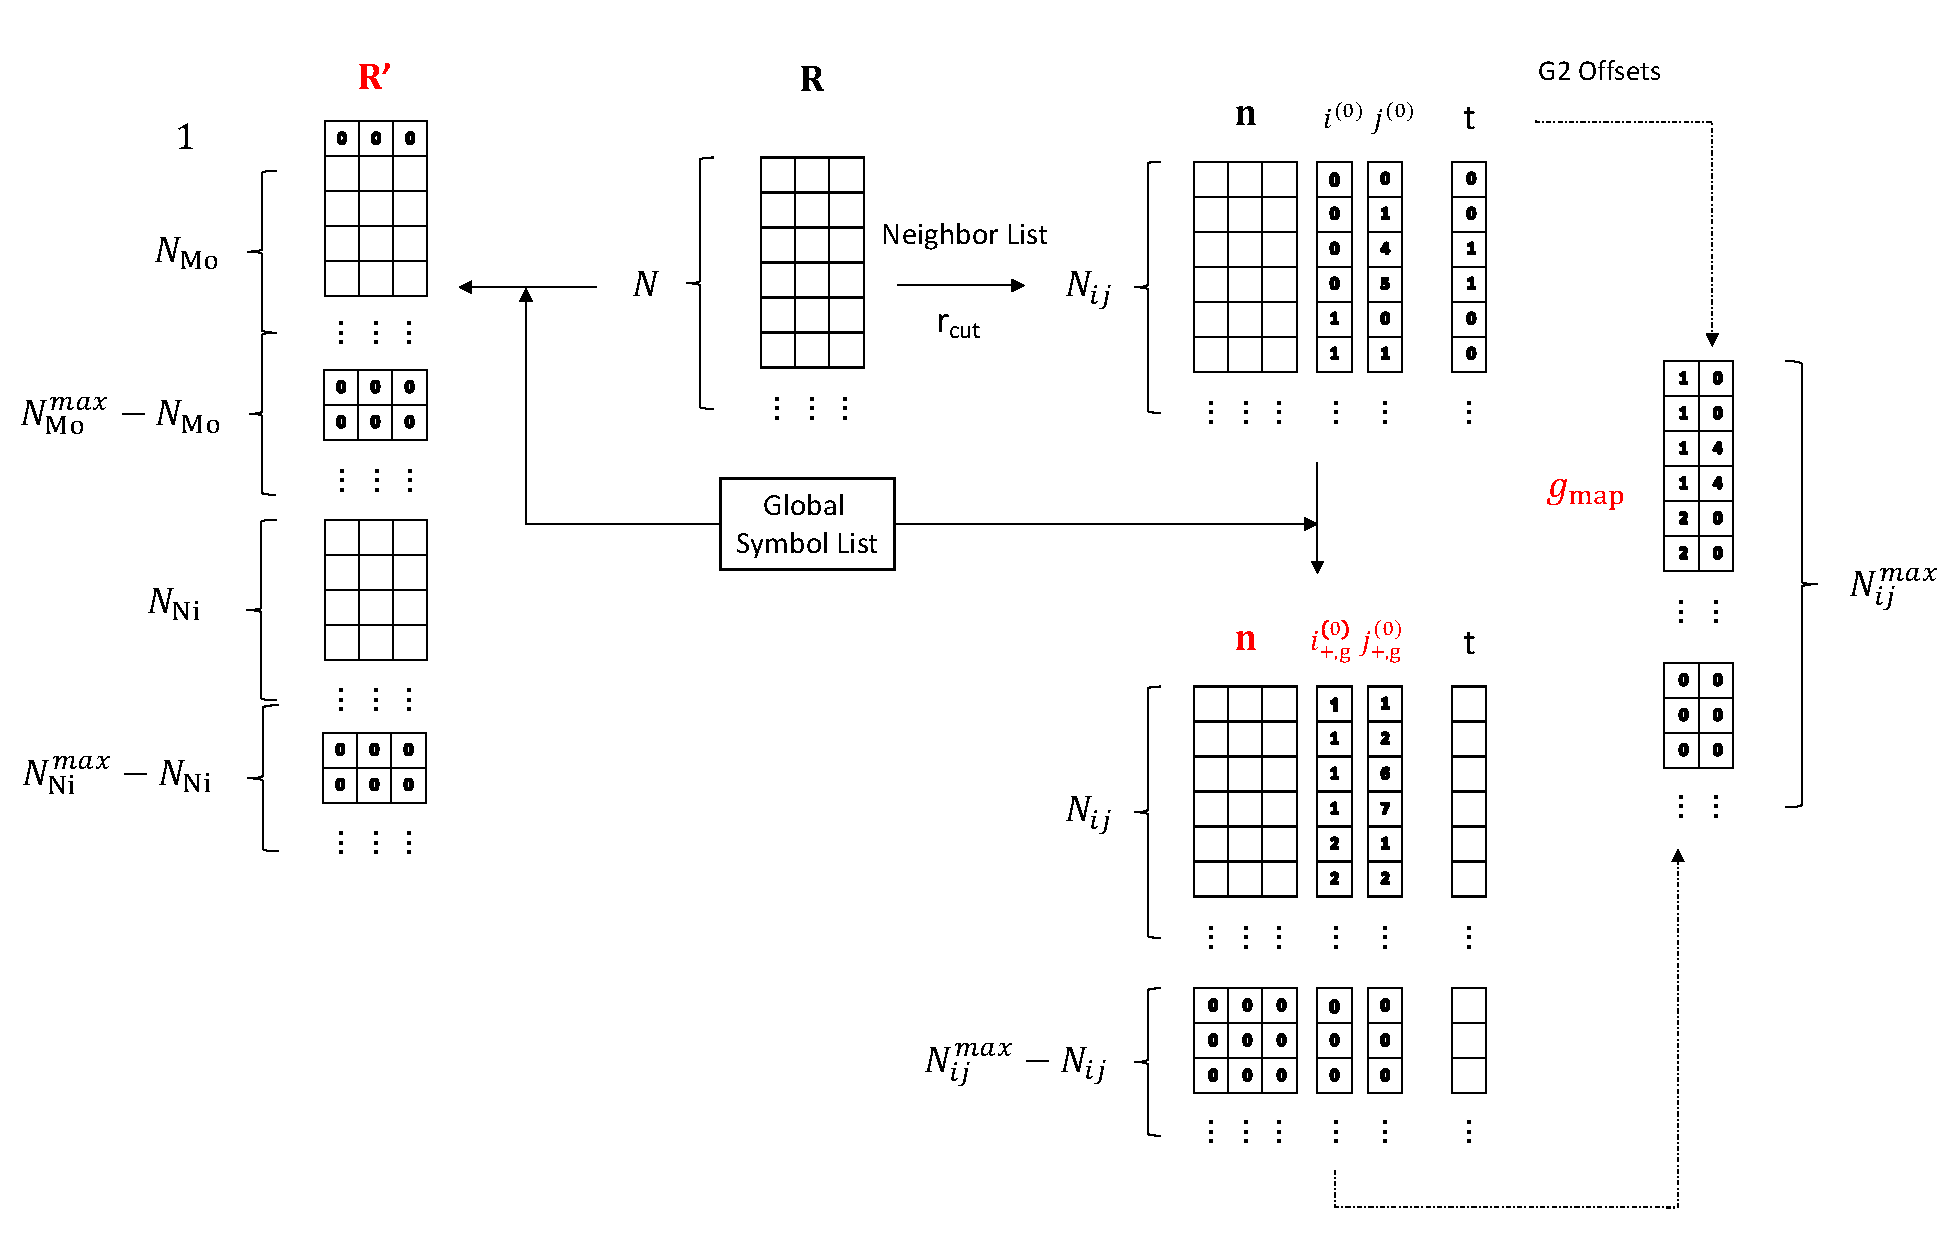
\includegraphics[scale=0.6]{figures/Fig2-v2gmap.pdf}
\caption{\label{fig:algo2} The second stage of the virtual atom approach: the 
construction of $g_{\mathrm{map}}^{(2)}$. Tensors marked red can be pre-computed 
and cached.}
\end{figure}

Fig \ref{fig:algo3} shows the final stage of the virtual atom approach: the 
computation graph for calculating radial symmetry function descriptors. This 
stage also starts from the $N \times 3$ local positions matrix \textbf{R} and 
involves two steps: the calculation of interatomic distances $r_{ij}$ 
(Fig \ref{fig:algo3}a) and the construction of $\mathbf{G}^{(2)}$ 
(Fig \ref{fig:algo3}b).

The initial step is to map local positions \textbf{R} to
$(N_{\mathrm{Ni}}^{\mathrm{max}}+N_{\mathrm{Mo}}^{\mathrm{max}}+1) \times 3$
global positions \textbf{R'} based on GSL. The first row (marked blue) of 
$\mathbf{R'}$ are all zeros representing 'positions' of the virtual atom. 
Then with 
\href{https://www.tensorflow.org/versions/r1.12/api_docs/python/tf/gather}
{tf.gather}, the global indices $i^{(0)}_{\mathrm{+,g}}$ and 
$j^{(0)}_{\mathrm{+,g}}$ of Fig \ref{fig:algo2} can be transformed to global 
positions: $\mathbf{R'_i}$ and $\mathbf{R'_j}$. Thus, the interatomic distances 
$r_{ij}$ can be simply calculated with Equation \ref{eq:rijn}.

Now it's time to get radial symmetry function descriptors matrix 
$\mathbf{G}^{(2)}$. 
As shown in Fig \ref{fig:algo3}b, this step can be executed in parallel: 
for each $\eta_i$, we first calcualte $g_2(r_{ij}, \eta_i)$ with 
Equation \ref{eq:g2} and then map the $N_{ij}^{\mathrm{max}}$-length vector 
$g_2(r_{ij}, \eta_i)$ to 
$(N_{\mathrm{Ni}}^{\mathrm{max}}+N_{\mathrm{Mo}}^{\mathrm{max}}+1) \times 16$ 
matrix $\mathbf{G}^{(2)}_{\eta_i}$ with $g^{\eta_i}_{\mathrm{map}}$ and 
\href{https://www.tensorflow.org/versions/r1.12/api_docs/python/tf/scatter_nd}
{tf.scatter\_nd}. Here $16$ is the multiplacation of 4 ($\eta$) and 4 
(radial interactions). 
$g^{\eta_i}_{\mathrm{map}}$ is calculated by adding a constant
$i - 1$ to all values of the second column of $g^{(2)}_{\mathrm{map}}$. Only 
shaded columns in Fig \ref{fig:algo3}b have non-zero values.
In fact, the first column of $g^{\eta_i}_{\mathrm{map}}$ means the indices of 
the central atoms in Equation \ref{eq:G2} (or rows of $\mathbf{G}^{(2)}$) and 
the second column marks the corresponding $\eta_i$ in Fig \ref{fig:algo1} (or 
columns of $\mathbf{G}^{(2)}$).
The first row of each $\mathbf{G}^{(2)}_{\eta_i}$ reprsents the descriptors of 
the virtual atom. Removing these rows with
\href{https://www.tensorflow.org/versions/r1.12/api_docs/python/tf/split}
{tf.split}, we get $\hat{\mathbf{G}}^{(2)}_{\eta_i}$.
The final radial symmetry function descriptors, $\mathbf{G}^{(2)}$ is just the 
sum of all $\hat{\mathbf{G}}^{(2)}_{\eta_i}$.

\begin{figure*}[h!]
\centering
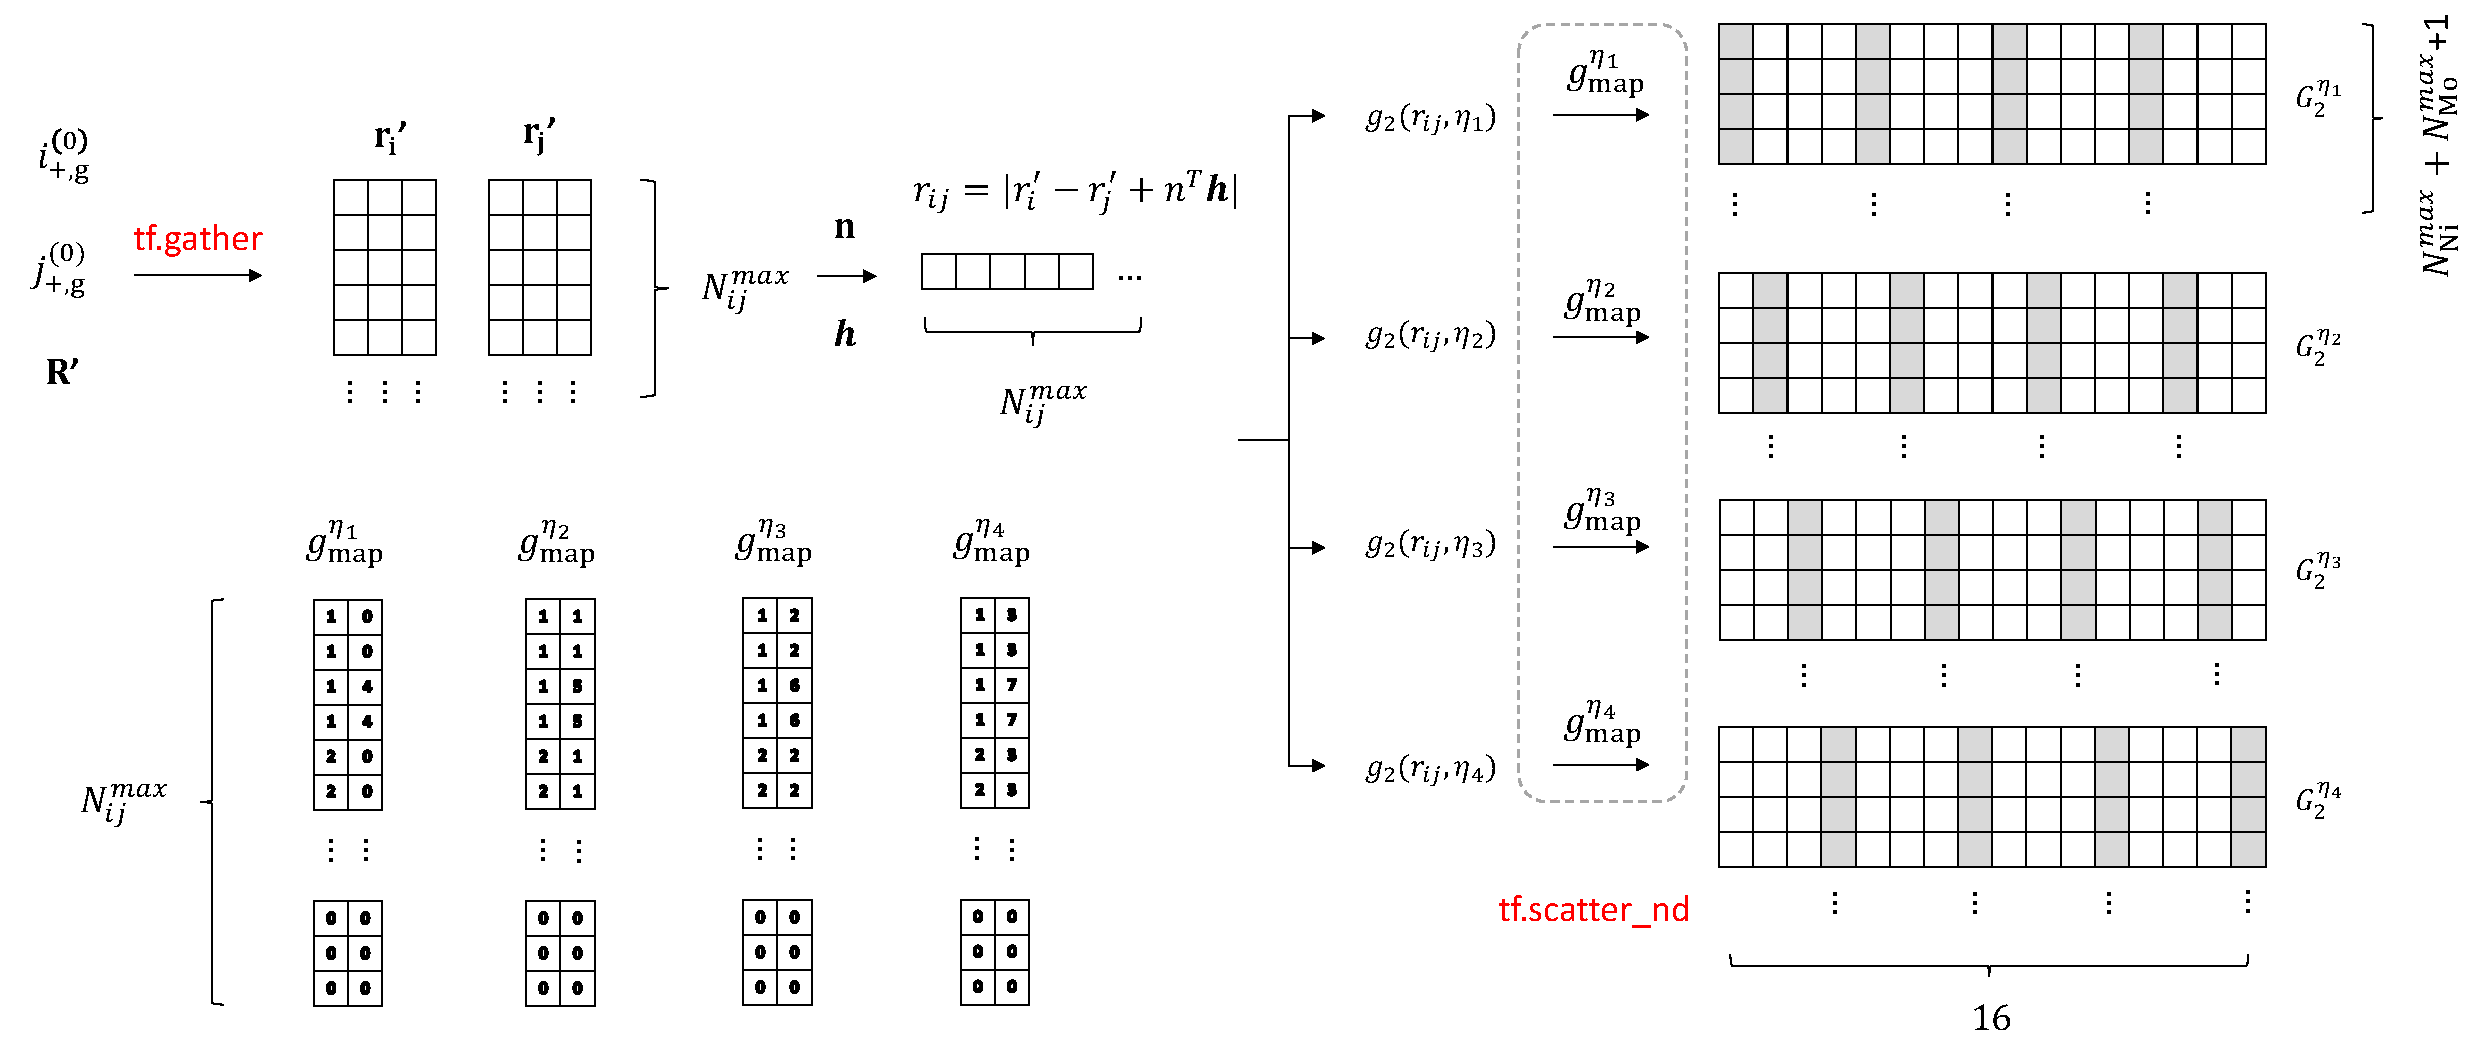
\includegraphics[scale=0.5]{figures/Fig3-G2.pdf}
\caption{\label{fig:algo3} 
\textbf{a)} The calculation of the interatomic distances $r_{ij}$.
\textbf{b)} The construction of the radial symmetry function descriptors 
$\mathbf{G}^{(2)}_{\eta_i}$. Rows that are marked blue correspond to the virtual 
atom and will be discared before feeding $\mathbf{G}$ into atomistic neural 
networks.
}
\end{figure*}

\subsection{The data flow}

The following equation briefly demonstrates the core data flow of 
\textbf{TensorAlloy} during a mini-batch training: 
\begin{equation}
    \mathbf{R'_{b}} \rightarrow 
    \mathbf{G_b} \rightarrow 
    \mathbf{E_b} \rightarrow
    \mathbf{F_b} \rightarrow 
    \mathbf{\epsilon_b} \rightarrow
    \mathbf{Loss}
\end{equation}
where the $N_{b} \times (\nmax + 1) \times 3$ matrix $\mathbf{R'_b}$ is a batch 
of positions matrices ($N_b \ge 1$ is the batch size), $\mathbf{G_b}$ is the 
corresponding symmetry function descriptors matrix of shape 
$N_{b} \times (\nmax) \times 16$ and $\mathbf{E_b}$ represents 
total energies of the structures. Section \ref{section:virtual_atom_approach} 
describes the implementation of $\mathbf{R'_{b}} \rightarrow \mathbf{G_b}$. 
To implement $\mathbf{G_b} \rightarrow \mathbf{E_b}$, \textbf{TensorAlloy} uses 
1D-convolutional neural networks with $1 \times 1$ kernels\cite{kCON}. The total 
forces $\mathbf{F_{b}}$ and the virial stress $\mathbf{\epsilon_{b}}$ are 
calculated with Equation \ref{eq:dEdr} and Equation \ref{eq:stress} directly.

\subsection{The residual model}

To fit the total energy, we slightly modified the total energy expression of 
Equation \ref{eq:general_e_total}:
\begin{align}
\label{eq:e_total_res}
E^{total} & = E^{residual} + E^{static} \nonumber \\
& = \sum_{i=1}^{N}{
    \mathbf{NN}_{el}\left( \left\{ G_i \right\} \right)
} + \sum_{el}{n_{el}E_{el}}
\end{align}
where $\{E_{el}\}$ is a set of \textit{trainable} scalar variables representing 
the \textit{static} energy of each type of element\cite{kCON}. The NN in 
Equation \ref{eq:e_total_res} just describes the atomistic interactions 
(the \textit{residual} energy). The 
introduction of $E^{static}$ can significantly limit value range of NN outputs, 
leading to faster convergence speed and higher training stability 
(Fig \ref{fig:benchmark_qm7}c). The initial $\{E_{el}\}$ are calculated by 
solving the linear system $Ax=b$ where $A$ is a $N_{data} \times N_{el}$ matrix 
and $b$ is a $N_{data}\times 1$ vector. $A(i,j)$ is the number of $j^{th}$
element in structure $i$ and $b(i)$ is the total energy of structure $i$.

To train the model, we use the following total loss function:
\begin{align}
\label{eq:loss}
\mathbf{Loss} & = \sqrt{\frac{1}{N_{b}}\sum_{i=1}^{N_{b}}{\left(
    E_{i} - E_{i}^{\mathrm{dft}}
\right)^2}} \nonumber \\
& + \chi_{\mathrm{f}}\sqrt{
    \frac{1}{3\sum_{i}^{N_{b}}{N_i}}\sum_{i}^{N_b}{\sum_{j}^{N_i}{
        \sum_{\alpha}{
            \left(f_{ij\alpha} - f_{ij\alpha}^{\mathrm{dft}}\right)^2
        }
    }}
} \nonumber \\
& + \chi_{\mathrm{s}}\sqrt{\frac{1}{6N_b}\sum_{i}^{N_b}{
    \sum_{j}^{6}{
        \left(
            \epsilon^{\mathrm{voigt}}_{j} - \epsilon^{\mathrm{voigt,dft}}_{j}
        \right)^2
    }
}}
\end{align}
where $N_b$ is the mini-batch size, $N_i$ is the number of atoms of structure 
$i$ and $\chi_{\mathrm{f}}$ and $\chi_{\mathrm{s}}$ are weights of force and 
stress losses. Typically both $\chi_{\mathrm{f}}$ and $\chi_{\mathrm{s}}$ range 
within $[1,10]$. Stress tensors are converted to Voigt vectors. All energies are 
in \textbf{eV}, all forces are in \textbf{eV/\AA} and all stress components are 
in \textbf{eV/\AA}$\mathbf{^3}$. In most cases, we set $N_b$ to 50 or 100 and we
use the ADAM\cite{adam} optimizer with exponentially-decayed learning rate to 
minimize the loss function. The activation function is Leaky ReLU
\cite{maas2013rectifier}:
\begin{equation}
\sigma(x) = \begin{cases}
    \alpha x & x \le 0 \\
    x & x \ge 0 \\
\end{cases}
\end{equation}
and $\alpha$ is set to 0.2 in \tensoralloy{}. The kernel weights of all ANNs are 
initialized with the Xvaier\cite{pmlr-v9-glorot10a} method and kernel biases are 
initialized with zeros.

% % % % % % % % % % % % % % % % % % % % % % % % % % % % % % % % % % % % % % % %
% 
% Section 4. Discussions
%
% % % % % % % % % % % % % % % % % % % % % % % % % % % % % % % % % % % % % % % %
\section{Discussions}
\label{section:discussions}

In this section we demonstrate two training experiments of \tensoralloy{}. All 
the results are obtained on a workstation with two Intel Xeon E5-2687v4 CPUs 
(18 cores per CPU, 2.3 GHz) and one NVIDIA GTX 1080 Ti GPU.

\subsection{QM7}

QM7\cite{QM7_1,QM7_2} is a publicly available benchmark dataset calculated at 
the DFT level. The QM7 dataset contains 7165 stable organic molecules 
(C, H, N, O, S) with 176 unique stoichiometries. The total energies range from 
-95 eV to -17 eV and the structure sizes range from 5 to 23. 1000 structures 
were randomly selected as test set before training.

Figure \ref{fig:benchmark_qm7} demonstrates the performances of 
\textbf{TensorAlloy} on QM7 dataset. In this figure, 'Radial' means only radial 
symmetry functions (Equation \ref{eq:G2}) are used and 'Angular' indicates both 
radial and angular symmetry functions are used. The cutoff radius is 6.5 \AA.
The corresponding $\nijmax$ and $\nijkmax$ are 506 and 5313, respectively, 
indicating the calculation of angular descriptors is much more expensive.
Values of $\eta$ for radial symmetry functions are 0.1, 0.5, 1, 2, 4, 8, 12, 16, 
20, 40 and $\beta$ (0.1, 0.5), $\gamma$ (1, -1) and $\zeta$ (1, 4) are used for
angular functions. $R_s$ is fixed to zero. The initial learning rate is 0.01 and 
then it is exponentially decayed with rate 0.99 for every 5000 steps. 
Each atomistic neural network has two hidden layers with 128 and 64 neurons.

Figure \ref{fig:benchmark_qm7}a compares the training speed (number of processed 
structures per second) with different batch sizes (number of structures per 
step). It shows that CPU perfers fewer descriptors (radial only) and smallber 
batch size while GPU is suitable for larger batch size and more complicated 
descriptors (radial + angular). 
Figure \ref{fig:benchmark_qm7}b shows the curves of mean absolute errors 
(MAEs, meV/atom) on the test set. This figure clearly illustrate another benefit 
of using larger batch size: models can be trained much faster. For the best case 
(batch size 100, angular symmetry functions included), the test MAE will reach 5 
meV/atom (1.5 kcal/mol per structure) within just one GPU hour. 

Figure \ref{fig:benchmark_qm7}c compares out residual model (Equation 
\ref{eq:e_total_res}) with traditional ANN model (Equation 
\ref{eq:general_e_total}). In fact, both models can converge to similar final 
results. However, the residual model has a much faster convergence speed because 
the introduction of the \textit{static} part can reduce output values of ANNs
close to (-1, 1) \textemdash the ideal output range of neural networks.

\begin{figure}[h!]
\centering
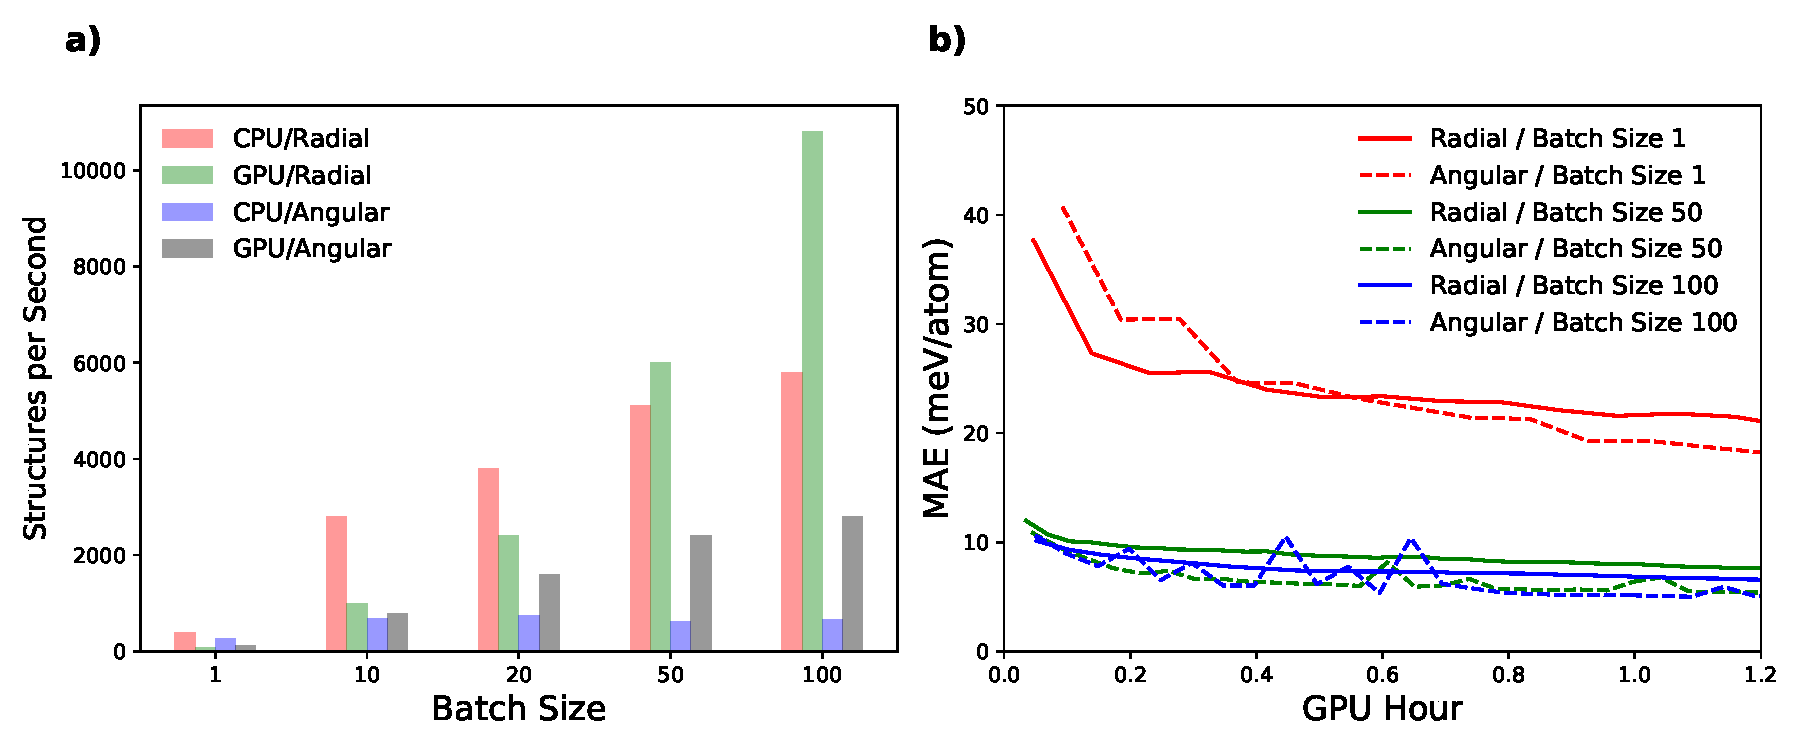
\includegraphics[scale=0.54]{figures/Fig4-qm7.pdf}
\caption{\label{fig:benchmark_qm7} 
\textbf{a)} The curves of training speed (structures per second) vs batch sizes. 
\textbf{b)} The curves of test MAE (meV/atom) vs training time (GPU hour) using 
different settings.
\textbf{c)} The curves of test MAE (meV/atom) vs NN models. 
}
\end{figure}

\subsection{Ni-Mo}

SNAP/Ni-Mo\cite{SNAP_Mo_2017, SNAP_2018} is a publicly available dataset built 
by Shyue Ping Ong and co-workers. This dataset has 3971 Ni-Mo solids, including 
461 pure Ni structures and 284 pure Mo structures. 
$N_{\mathrm{Ni}}^{\mathrm{max}}$ is 108 and $N_{\mathrm{Mo}}^{\mathrm{max}}$ 
equals 176. All DFT calculations were done by VASP\cite{VASP} using the 
PBE\cite{PBE} functional within the projector angumented-wave (PAW)\cite{PAW} 
approach.

In this experiment, we trained four different models:
\begin{enumerate}
    \item SFNN/Ni: this model uses 400 Ni structures for training and 61 for 
    evaluation. The loss function only includes energy and force. Hidden layer 
    settings are 128,64,32.
    \item SFNN/Mo: this model uses 250 Mo structures for training and 34 for 
    evaluation. The loss function includes all three metrics. Hidden layer 
    settings are also 128,64,32.
    \item SFNN/Ni-Mo: this model uses 3600 randomly selected structures for 
    training and the rest 373 structures are used for evaluation. The loss 
    function includes only energy and force. Hidden layer settings are 64,32,32.
    \item SFNN/Ni-Mo (esf): this model has exactly the same settings with 
    SFNN/Ni-Mo except that its loss function also includes stress as training 
    metrics. $\chi_{s}$ of Equation \ref{eq:loss} is 160.
\end{enumerate}

For all these models, the cutoff radius is set to 6.0 \AA. The $\nijmax$ for Ni, 
Mo and Ni-Mo are 4678, 4504 and 7200, respectively. Only radial symmetry 
functions are used to compute atomic descriptors. The selected $\eta$ are: 
0.1, 0.5, 1, 2, 4, 8, 12, 16, 20 and 40. The learning rate starts from 0.01 and 
it will decay exponentially with rate 0.99 for every 5000 training steps. The
maximum training steps is 500,000.

\begin{table}[h]
\centering
\begin{tabular}{lcccccccc}
\hline
    & Model & Mo & Ni$_4$Mo & Ni$_3$Mo & Ni$_{\mathrm{Mo}}$ & Mo$_{\mathrm{Ni}}$ 
    & Ni & Overall \\
\hline
Energy (meV/atom) & Ni SNAP & & & & & & \textbf{1.2} & \\
    & Mo SNAP & 13.2 & & & & & & \\
    & Ni-Mo SNAP & 16.2 & 4.0 & 5.2 & 22.7 & 33.9 & 7.9 & 22.5 \\
    & Ni SFNN & & & & & & 1.6 & \\
    & Mo SFNN & \textbf{9.8} & & & & & & \\
    & Ni-Mo SFNN & 22.1 & \textbf{3.3} & \textbf{4.1} & \textbf{11.3} 
    & \textbf{13.7} & 3.7 & \textbf{11.0} \\
    & Ni-Mo SFNN (esf) & 30.0 & 6.1 & 9.0 & 16.6 
    & 26.2 & 7.8 & 19.1 \\
\hline
Force (eV/\AA) & Ni SNAP & & & & & & 0.05 & \\
& Mo SNAP & 0.25 & & & & & & \\
& Ni-Mo SNAP & 0.29 & 0.14 & 0.16 & 0.13 & 0.55 & 0.11 & 0.23 \\
& Ni SFNN & & & & & & \textbf{0.05} & \\
& Mo SFNN & \textbf{0.20} & & & & & & \\
& Ni-Mo SFNN & 0.32 & \textbf{0.09} & 0.11 & 0.09 & 
    \textbf{0.15} & 0.06 & 0.12 \\
& Ni-Mo SFNN (esf) & 0.36 & 0.10 & \textbf{0.11} & \textbf{0.08} & 
    0.16 & 0.06 & \textbf{0.12} \\
\hline
Stress (GPa) & Mo SNAP & \textbf{0.87} & & & & & & \\
& Mo SFNN & 1.00 & & & & & & \\
& Ni-Mo SFNN & 5.77 & \textbf{1.72} & 1.74 & 1.45 & 3.75 & 1.97 & 2.83 \\
& Ni-Mo SFNN (esf) & \textbf{1.84} & 2.05 & \textbf{1.38} & \textbf{0.57} & 
    \textbf{1.22} & \textbf{1.91} & \textbf{1.27} \\
\hline
\end{tabular}
\caption{\label{table:MAE}
Comparion of the MAEs in predicted energies (mev/atom), forces (eV/\AA) and 
stress (GPa) relative to DFT for the \tensoralloy{} models and their 
corresponding SNAP models}
\end{table}

\begin{figure}[h!]
    \centering
    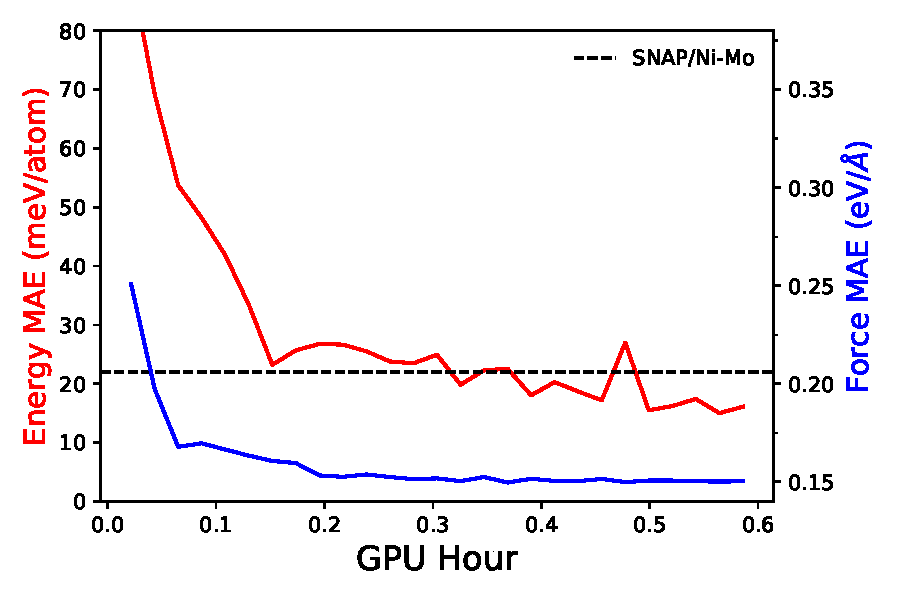
\includegraphics[scale=0.8]{figures/Fig5-snap.pdf}
\caption{\label{fig:snap_gpu_train_speed} The test MAEs of the SFNN/Ni-Mo model 
vs training time (GPU Hour). The black dotted line marks the final performance 
of the SNAP/Ni-Mo model \cite{SNAP_2018}.}
\end{figure}

Table \ref{table:MAE} summarizes the energy, force and stress prediction 
performances of \tensoralloy{}-optmized models compared with their corresponding 
SNAP models. The original SNAP formalism contains both radial and angular 
interactions. However, in most cases, the radial-only \tensoralloy{}-trained 
SFNN models can significantly outperform corresponding SNAP models. To precisely
predict virial stress, integrating stress into total loss is undoubtedly 
necessary. For the pure Mo dataset, the SFNN/Mo model gives a MAE of 1.0 GPa on 
predicting stress while it will increase to 2 GPa if only using energy and force 
as training metrics. This phonomenon holds true for the Ni-Mo mixed models as 
well. If we include stress in the total loss function, we can obtain much more 
accurate stress predictions.

The trainings of \tensoralloy{} on these \textit{solid} datasets are also very 
fast. Fig \ref{fig:snap_gpu_train_speed} shows the test MAE (meV/atom) vs 
training time (GPU Hour) of the SFNN/Ni-Mo model. \tensoralloy{} only needs less 
than \textbf{half an hour} to achieve equivalent performance of the 
SNAP/Ni-Mo model.

\begin{figure}[h!]
    \centering
    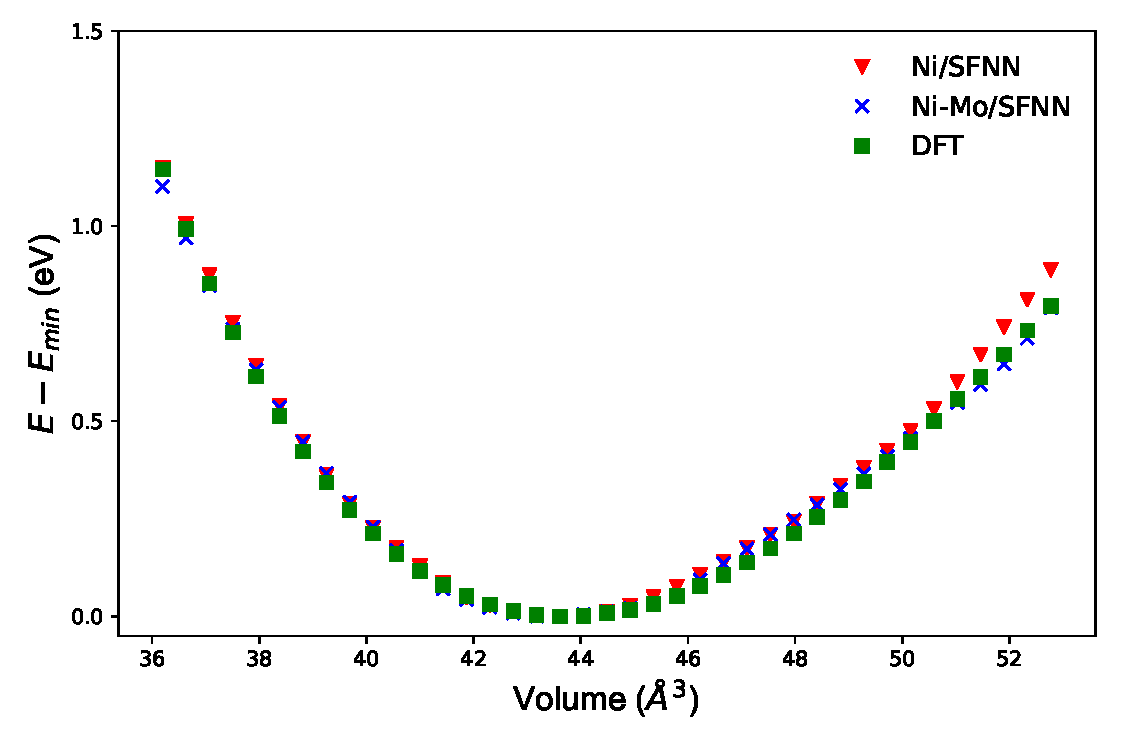
\includegraphics[scale=0.8]{figures/Fig6-energy-volume.pdf}
\caption{\label{fig:energy_volume_Ni} The energy vs volume curves of fcc Ni for
the DFT, Ni/SFNN and Ni-Mo/SFNN models.}
\end{figure}

To further validate our models, we also calculate the energy-volume curves of a 
conventional fcc Ni cell using SFNN/Ni and SFNN/Ni-Mo models. The results are 
plotted in Fig \ref{fig:energy_volume_Ni}. Both curves overlap the DFT curve 
very well in the range of -17\% to 21\% from the equilibrium volume. The surface
energy tests, as shown in Fig \ref{fig:surface_energy_Ni}, also proves the 
accuracy of TensorAlloy-optimized models. PyMatGen\cite{pymatgen,pymatgen-1} is 
used to generate these surface slabs.

\begin{figure}[h!]
    \centering
    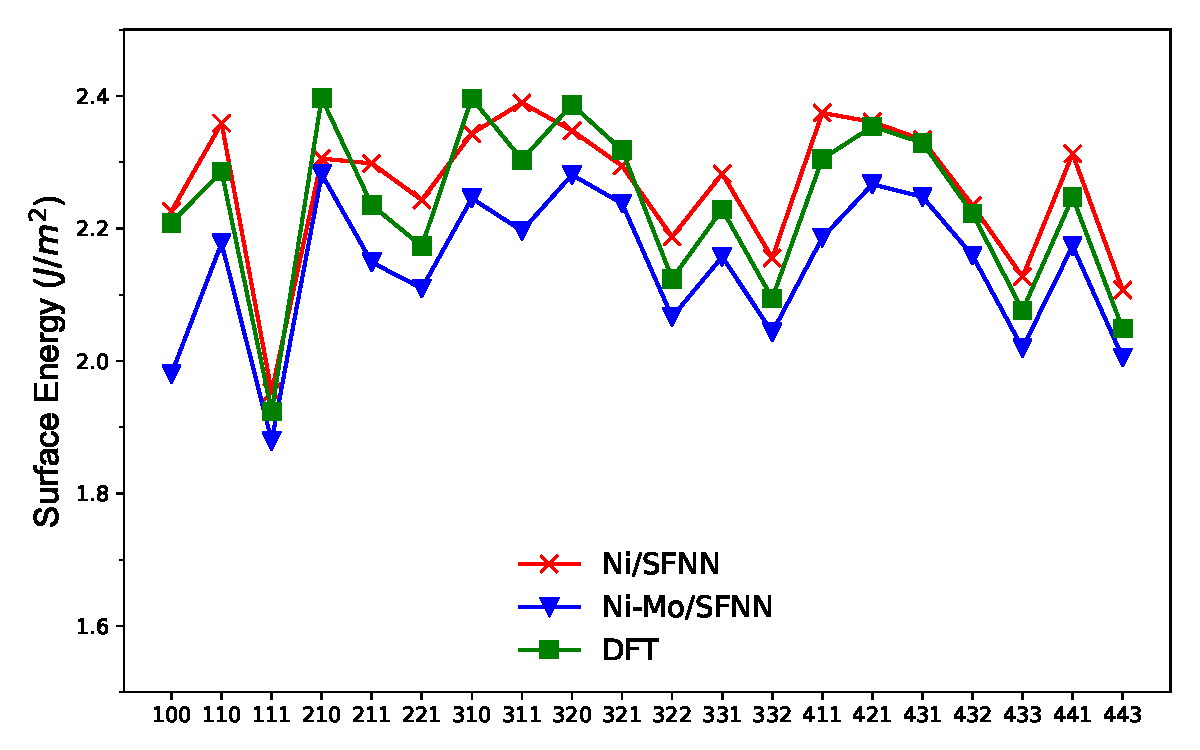
\includegraphics[scale=0.8]{figures/Fig7-surface-energy.pdf}
\caption{\label{fig:surface_energy_Ni} Surface formation energies ($J/m^2$) of 
different Ni surfaces calculated by DFT, Ni/SFNN and Ni-Mo/SFNN models. 
The MAEs of the Ni/SFNN and Ni-Mo/SFNN relative to the DFT values are 0.09 and 
0.05, respectively.}
\end{figure}

% % % % % % % % % % % % % % % % % % % % % % % % % % % % % % % % % % % % % % % %
% 
% Section 5. Conclusions
%
% % % % % % % % % % % % % % % % % % % % % % % % % % % % % % % % % % % % % % % %
\section{Conclusions}
\label{section:conclusions}

In this work, we proposed a new algorithm, namd the virtual atom approach, 
to construct symmetry function based atomistic neural networks. With this 
method, we can build direct computation graph from positions to total energy 
using modern machine learning frameworks (like TensorFlow), thus, making the 
technical barrier of calculating NN-derived atomic force and virial stress  
neglectable. We also derived an alternative form of the general virial stress 
equation. The new formula can be implemented with simple matrix operations and 
is suitable for arbitrary machine learning platform based potentials. We 
developed a highly efficient Python program, \tensoralloy{, for both 
\textit{molecules} and \textit{solids}. We tested our program on two public 
datasets, QM7 (molecules) and SNAP/Ni-Mo (solids). \tensoralloy{} can reach 
state-of-art performances within just one GPU Hour.

% % % % % % % % % % % % % % % % % % % % % % % % % % % % % % % % % % % % % % % %
% 
% Acknowledgments
%
% % % % % % % % % % % % % % % % % % % % % % % % % % % % % % % % % % % % % % % %
\section*{Acknowledgments}

This work was supported by the National Key Research and Development Program of 
China under Grant No. 2016YFB0201203, the Science Challenge Project under Grant 
No. TZ2018002 and the National Natural Science Foundation of China under Grant 
No. U1630250.

% % % % % % % % % % % % % % % % % % % % % % % % % % % % % % % % % % % % % % % %
% 
% References
%
% % % % % % % % % % % % % % % % % % % % % % % % % % % % % % % % % % % % % % % %
\bibliography{manuscript.bib}

\newpage

% % % % % % % % % % % % % % % % % % % % % % % % % % % % % % % % % % % % % % % %
% 
% Appendix
%
% % % % % % % % % % % % % % % % % % % % % % % % % % % % % % % % % % % % % % % %
\section*{Appendix}
\label{section:appendix}

\subsection{
    Calculations of $N_{ij}^{\mathrm{max}}$ and $N_{ijk}^{\mathrm{max}}$}

The following codes shows how to calculate $N_{ij}^{\mathrm{max}}$ and 
$N_{ijk}^{\mathrm{max}}$. Python-3.7 and ASE-3.17.0 are suggested. In this block
\textmd{dataset} should be a list of \textmd{ase.Atoms} objects.
\begin{verbatim}
nij_max = 0
nijk_max = 0
for i in range(dataset):
    atoms = dataset[i]
    assert isinstance(atoms, ase.Atoms)
    ilist, jlist = ase.neighborlist.neighbor_list('ij', atoms, cutoff=rc)
    nij = len(ilist)
    nl = {}
    for i, atomi in enumerate(ilist):
        if atomi not in nl:
            nl[atomi] = []
        nl[atomi].append(jlist[i])
    nijk = 0
    for atomi, nlist in nl.items():
        n = len(nlist)
        nijk += (n - 1 + 1) * (n - 1) // 2
    nij_max = max(nij, nij_max)
    nijk_max = max(nijk, nijk_max)
\end{verbatim}

\subsection{Derivation and implementation of the virial stress equation}

According to Equation \ref{eq:lattice} and Equation \ref{eq:ij_shift}, Equation 
\ref{eq:rijn} can be expanded:
\begin{align}
\rijn = & \Vert \mathbf{r}_i^{(0)} - \mathbf{r}_j^{(0)} + 
           \mathbf{n}^T \mathbf{h} \Vert \nonumber \\
      = & \left[
                 \left(r_{j,x}^{(0)} - r_{i,x}^{(0)} + 
                       \sum_{\alpha}{n_{\alpha}h_{\alpha x}} \right)^2 +
                 \left(r_{j,y}^{(0)} - r_{i,y}^{(0)} + 
                       \sum_{\alpha}{n_{\alpha}h_{\alpha y}} \right)^2 + \right.
        \nonumber \\
        & \left. \left(r_{j,z}^{(0)} - r_{i,z}^{(0)} + 
                       \sum_{\alpha}{n_{\alpha}h_{\alpha z}} \right)^2 
          \right]^{\frac{1}{2}}
\end{align}
where $\alpha=x,y,z$. Thus, we can calculate the derivation of $\rijn$ with 
respect to $h_{\alpha\beta}$:
\begin{gather}
\frac{\partial \rijn}{\partial h_{\alpha\beta}} = 
    \frac{1}{\rijn} \cdot \Delta_{ij\mathbf{n}\beta} \cdot n_{\alpha} \\
\Delta_{ij\mathbf{n}\beta} = r_{j,\beta}^{(0)} - r_{i,\beta}^{(0)} + 
    \sum_{\alpha}{n_{\alpha}h_{\alpha \beta}}
\end{gather}

\newcommand{\hab}{h_{\alpha\beta}}
\newcommand{\hga}{h_{\gamma\alpha}}
\newcommand{\hgb}{h_{\gamma\beta}}

Then we can derive $\partial E^{total} / \partial \hab$:
\begin{align}
\label{eq:dEdhab}
\frac{\partial E^{total}}{\partial \hab} = \sum_{i}^{N}{\sum_{l}^{N_G}}{
    \frac{\partial \mathbf{NN}_{el}(\mathbf{G}_i)}{\partial G_{il}}
    \cdot
    \frac{\partial G_{il}}{\partial \hab}
}
\end{align}
If $G_{il}$ is a radial symmetry function:
\begin{align}
\frac{\partial G_{il}^{(2)}}{\partial \hab} 
& = \sum_{j \neq i}{\sum_{\mathbf{n}}}{
    \frac{\partial g_2}{\partial \rijn} 
    \cdot 
    \frac{1}{\rijn} \cdot \Delta_{ij\mathbf{n}\beta} \cdot n_{\alpha}
} \\
\label{eq:stress_g2_right}
\frac{\partial G_{il}^{(2)}}{\partial \hga} \cdot \hgb & = 
\sum_{j \neq i}{\sum_{\mathbf{n}}}{
    \frac{\partial g_2}{\partial \rijn} 
    \cdot 
    \frac{\Delta_{ij\mathbf{n}\alpha}}{\rijn} \cdot n_{\gamma}
} \cdot \hgb
\end{align}
If $G_{il}$ is an angular symmetry function:
\begin{align}
\frac{\partial G_{il}^{(4)}}{\partial \hab} & =
    \sum_{j, k \neq j, k \neq i}{
        \sum_{\mathbf{n_1}}}{\sum_{\mathbf{n_2}}{\sum_{\mathbf{n_3}}{
    \left(
        \frac{\partial g_4}{\partial \rijna}\cdot\frac{\partial \rijna}{\hab} +
        \frac{\partial g_4}{\partial \rikna}\cdot\frac{\partial \rikna}{\hab} +
        \frac{\partial g_4}{\partial \rjkna}\cdot\frac{\partial \rjkna}{\hab}
    \right)
}}} \nonumber \\
& =  \sum_{j, k \neq j, k \neq i}{
        \sum_{\mathbf{n_1}}}{\sum_{\mathbf{n_2}}{\sum_{\mathbf{n_3}}{
    \frac{\partial g_4}{\partial \rijna} \cdot 
    \frac{\Delta_{ij\mathbf{n_1}\beta}}{\rijna} \cdot n_{1,\alpha}
}}} \nonumber \\
& + \sum_{j, k \neq j, k \neq i}{
    \sum_{\mathbf{n_1}}}{\sum_{\mathbf{n_2}}{\sum_{\mathbf{n_3}}{
\frac{\partial g_4}{\partial \rikna} \cdot 
\frac{\Delta_{ik\mathbf{n_2}\beta}}{\rikna} \cdot n_{2,\alpha}
}}} \nonumber \\
& + \sum_{j, k \neq j, k \neq i}{
    \sum_{\mathbf{n_1}}}{\sum_{\mathbf{n_2}}{\sum_{\mathbf{n_3}}{
\frac{\partial g_4}{\partial \rjkna} \cdot 
\frac{\Delta_{jk\mathbf{n_2}\beta}}{\rjkna} \cdot n_{3,\alpha}
}}} \\
\label{eq:stress_g4_right}
\frac{\partial G_{il}^{(4)}}{\partial \hga} \cdot \hgb & = 
\sum_{j, k \neq j, k \neq i}{
    \sum_{\mathbf{n_1}}}{\sum_{\mathbf{n_2}}{\sum_{\mathbf{n_3}}{
\frac{\partial g_4}{\partial \rijna} \cdot 
\frac{\Delta_{ij\mathbf{n_1}\alpha}}{\rijna} \cdot n_{1,\gamma} \cdot \hgb
}}} \nonumber \\
& + \sum_{j, k \neq j, k \neq i}{
    \sum_{\mathbf{n_1}}}{\sum_{\mathbf{n_2}}{\sum_{\mathbf{n_3}}{
\frac{\partial g_4}{\partial \rikna} \cdot 
\frac{\Delta_{ik\mathbf{n_1}\alpha}}{\rikna} \cdot n_{2,\gamma} \cdot \hgb
}}} \nonumber \\
& + \sum_{j, k \neq j, k \neq i}{
    \sum_{\mathbf{n_1}}}{\sum_{\mathbf{n_2}}{\sum_{\mathbf{n_3}}{
\frac{\partial g_4}{\partial \rjkna} \cdot 
\frac{\Delta_{jk\mathbf{n_1}\alpha}}{\rjkna} \cdot n_{3,\gamma} \cdot \hgb
}}}
\end{align}
Combining with Equation \ref{eq:dEdhab}, \ref{eq:stress_g2_right} and 
\ref{eq:stress_g4_right}, we can now start deriving the right part of Equation 
\ref{eq:stress}. To simplify the derivation, we just assume $G_{il}$ represents
a radial function:
\newcommand{\dE}{\partial{E^{total}}}
\begin{align}
\label{eq:dEdhTh_g2_expanded}
\left(
    \left(\frac{\partial E^{total}}{\partial \mathbf{h}}\right)^T \mathbf{h}
\right)_{\alpha\beta} & = 
\sum_{\gamma}{\frac{\dE}{\partial \hga} \hgb} \nonumber \\
& = \sum_{\gamma}{\sum_{i}^{N}{\sum_{l}^{N_G}}{
    \frac{\partial \mathbf{NN}_{el}(\mathbf{G}_i)}{\partial G_{il}}
    \cdot
    \sum_{j \neq i}{\sum_{\mathbf{n}}}{
    \frac{\partial g_2}{\partial \rijn} 
    \cdot 
    \frac{\Delta_{ij\mathbf{n}\alpha}}{\rijn} \cdot n_{\gamma}} \hgb
}} \nonumber \\
& = \sum_{i}^{N}{\sum_{l}^{N_G}}{\sum_{j \neq i}{\sum_{\mathbf{n}}}{
    \frac{\partial \mathbf{NN}_{el}(\mathbf{G}_i)}{\partial G_{il}}
    \cdot
    \frac{\partial g_2}{\partial \rijn} 
    \cdot 
    \frac{\Delta_{ij\mathbf{n}\alpha}}{\rijn}}
    \sum_{\gamma}{\cdot n_{\gamma}\hgb}
} \nonumber \\
& = -\sum_{i}^{N}{\sum_{l}^{N_G}}{\sum_{j \neq i}{\sum_{\mathbf{n}}}{
    f^{'}_{ij\mathbf{n}\alpha}
    \sum_{\gamma}{\cdot n_{\gamma}\hgb}
}}
\end{align}
where $f^{'}_{ij\mathbf{n}}$ is the partial force:
\begin{equation}
f^{'}_{ij\mathbf{n}\alpha} = 
-\frac{\partial \mathbf{NN}_{el}(\mathbf{G}_i)}{\partial G_{il}} \cdot 
\frac{\partial g_2}{\partial \rijn} \cdot 
\frac{\Delta_{ij\mathbf{n}\alpha}}{\rijn}
\end{equation}
If $G_{il}$ is an angular symmetry function, we can also get a similar 
expression. Thus,
\begin{equation}
\left(\frac{\partial E^{total}}{\partial \mathbf{h}}\right)^T \mathbf{h} =
-\left(\sum_{\mathbf{n}}{\mathbf{h}^T\mathbf{n}} \otimes 
\sum_{i=1}^{N}{F^{\prime}_{i\mathbf{n}}}\right)^T
\end{equation}
The left part of Equation \ref{eq:stress} can be calculated with 
simple matrix multiplacation:
\begin{equation}
\sum_{i=1}^{N}{\mathbf{r}_i^{(0)} \otimes f_i} = R^{T} F
\end{equation}
So finally we can derive the vectorized expression of virial stress:
\begin{equation}
\epsilon = -F^{T} R + \left( \frac{\dE}{\partial \mathbf{h}} \right)^T\mathbf{h}
\end{equation}

Now, the virial stress can be calculated with just a few lines of codes within 
arbitrary Machine Learning framework (TensorFlow, PyTorch, etc). The following 
codes are written in Python-3.7/TensorFlow-1.12, where \textit{energy} and 
\textit{volume} are scalar tensors, \textit{cell} is a $3 \times 3$ tensor, 
\textit{positions} is a $N\times 3$ tensor and \textit{forces} (the total forces 
on these atoms) is also a $N\times 3$ tensor:
\begin{verbatim}
def get_virial_stress_tensor(energy, cell, volume, positions, forces):
    dEdh = tf.gradients(energy, cell, name='dEdh)[0]
    right = tf.matmul(tf.transpose(dEdh, name='dEdhT'), cell)
    left = tf.matmul(tf.transpose(forces), positions)
    stress = tf.add(tf.negative(left), right, name='stress')
    stress = tf.div(stress, volume, name='virial')
    return stress
\end{verbatim}

\newpage

\subsection{Implementation of the $g^2_{\mathrm{map}}$}

This function shows the calculation of $g^2_{\mathrm{map}}$. The returned dict
contains $g^2_{\mathrm{map}}$, $i^{(0)}_{\mathrm{+,g}}$, 
$j^{(0)}_{\mathrm{+,g}}$ and $\mathbf{n_g}$. $\nijmax$ should be provided in 
advance. \textmd{interactions} is a list of \textmd{string} representing the 
\textbf{ordered} interactions (e.g. \textmd{['NiNi','NiMo','MoMo','MoNi']}). 
\textmd{offsets} is a list of integers marking the starting indices of the 
\textmd{interactions}. As an example, if $N_{\eta}$ is 8, the \textmd{offsets}
corresponding to \textmd{['NiNi','NiMo','MoMo','MoNi']} should be 
\textmd{[0, 8, 16, 24]}.
\textmd{local\_to\_global\_map} is a dict mapping local indices to global 
indices.

\begin{verbatim}
def get_g2_map(atoms: Atoms, nij_max: int, interactions: list, 
               local_to_global_map: dict, offsets: list):
    g2_map = np.zeros((nij_max, 2), dtype=np.int32)
    tlist = np.zeros(nij_max, dtype=np.int32)
    symbols = atoms.get_chemical_symbols()
    ilist, jlist, Slist = neighbor_list('ijS', atoms, rc)
    nij = len(ilist)
    tlist.fill(0)
    for i in range(nij):
        symboli = symbols[ilist[i]]
        symbolj = symbols[jlist[i]]
        tlist[i] = interactions.index('{}{}'.format(symboli, symbolj))
    ilist = np.resize(ilist + 1, (nij_max, ))
    jlist = np.resize(jlist + 1, (nij_max, ))
    Slist = np.resize(Slist, (nij_max, 3))
    for count in range(len(ilist)):
        if ilist[count] == 0:
            break
        ilist[count] = local_to_global_map[ilist[count]]
        jlist[count] = local_to_global_map[jlist[count]]
    g2_map[:, 0] = ilist
    g2_map[:, 1] = offsets[tlist]
    return {"g2_map": g2_map, "ilist": ilist, "jlist": jlist, 
            "shift": np.asarray(Slist)}
\end{verbatim}

\newpage

\subsection{Implementation of the $g^4_{\mathrm{map}}$}

The construction of $g^4_{\mathrm{map}}$ is similar to $g^2_{\mathrm{map}}$. 
$\nijkmax$ should be provided in advance. 
\textmd{global\_to\_local\_map} is the reverse dict of 
\textmd{local\_to\_global\_map}.
\begin{verbatim}
def get_g4_map(atoms: Atoms, g2_map: dict, interactions: list, 
               offsets: list, global_to_local_map: dict, nijk_max: int):
    g4_map = np.zeros((nijk_max, 2), dtype=np.int32)
    ijk = np.zeros((nijk_max, 3), dtype=np.int32)
    n1 = np.zeros((nijk_max, 3), dtype=np.float32)
    n2 = np.zeros((nijk_max, 3), dtype=np.float32)
    n3 = np.zeros((nijk_max, 3), dtype=np.float32)
    symbols = atoms.get_chemical_symbols()
    indices = {}
    vectors = {}
    for i, atomi in enumerate(g2["ilist"]):
        if atomi == 0:
            break
        if atomi not in indices:
            indices[atomi] = []
            vectors[atomi] = []
        indices[atomi].append(g2["jlist"][i])
        vectors[atomi].append(g2["shift"][i])
    count = 0
    for atomi, nl in indices.items():
        indexi = global_to_local_map[atomi]
        symboli = symbols[indexi]
        prefix = '{}'.format(symboli)
        for j in range(len(nl)):
            atomj = nl[j]
            indexj = global_to_local_map[atomj]
            symbolj = symbols[indexj]
            for k in range(j + 1, len(nl)):
                atomk = nl[k]
                indexk = global_to_local_map[atomk]
                symbolk = symbols[indexk]
                interaction = '{}{}'.format(
                    prefix, ''.join(sorted([symbolj, symbolk])))
                ijk[count] = atomi, atomj, atomk
                n1[count] = vectors[atomi][j]
                n2[count] = vectors[atomi][k]
                n3[count] = vectors[atomi][k] - vectors[atomi][j]
                index = interactions.index(interaction)
                g4_map[count, 0] = atomi
                g4_map[count, 1] = offsets[index]
                count += 1
    return {"g4_map": g4_map, "ij": ij, "ik": ik, "jk": jk, 
            "n1": n1, "n2": n2, "n3": n3}
\end{verbatim}

\end{document}
